\section{Background}

\section{Approach}

\begin{figure}[!t]
\centering
% TikZ diagram for black-box safety validation problem formulation.
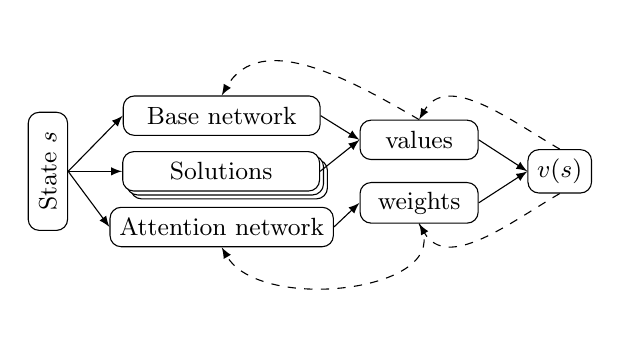
\begin{tikzpicture}
    \tikzstyle{every node}=[font=\small, align=center]
    \tikzset{
        n/.style={draw, rounded corners, minimum height=0.5cm, minimum width = 1.5cm},
        n2/.style={n, minimum width=2.5cm}
        }
    
    %state 
    \node (state) [n, rotate=90] {\small State $s$};
    
    %base network
    \node (base) [n2, above right of=state, xshift=1.5cm] {Base network};
    
    %Solutions
    \node (solutionsback1) [n2, right of=state, xshift=1.3cm, yshift=-0.1cm] {};
    \node (solutionsback2) [n2, fill=white, right of=state, xshift=1.25cm, yshift=-0.05cm] {};
    \node (solutions) [n2, fill=white, right of=state, xshift=1.2cm] {Solutions};
    
    %weights
    \node (attn) [n2, below right of=state, xshift=1.5cm] {Attention network};
    

    \node (values) [n, below right of=base, xshift=1.8cm, yshift = 0.4cm] {values};
    
     \node (weights) [n, above right of=attn, xshift=1.8cm, yshift = -0.4cm] {weights};
     
     \node (pfail) [n, minimum width = 0.5cm, right of=state, xshift=5.5cm] {$v(s)$};
    

    \draw[-latex] (state.south) -- (base.west);
    \draw[-latex] (state.south) -- (solutions.west);
    \draw[-latex] (state.south) -- (attn.west);
    
    \draw[-latex] (base.east) -- (values.west);
    \draw[-latex] (solutions.east) -- (values.west);
    \draw[-latex] (attn.east) -- (weights.west);
    
    \draw[-latex] (weights.east) -- (pfail.west);
    \draw[-latex] (values.east) -- (pfail.west);
    
    
    % backprop
    
    \draw [dashed, -latex] (weights.south) to [out=-1500,in=-60] (attn.south);
    \draw [dashed, -latex] (pfail.south) to [out=-150,in=-60] (weights.south);
    \draw [dashed, -latex] (values.north) to [out=150,in=60] (base.north);
    \draw [dashed, -latex] (pfail.north) to [out=150,in=60] (values.north);
\end{tikzpicture}
\caption{The A2T network. Dashed lines represent backpropagation for learning parameters. }
\label{fig:A2T_Network}
\vskip -0.5cm
\end{figure}

\begin{algorithm}
\caption{MC evaluation with function approximation}
    \label{alg:mc_policy_eval}
\begin{algorithmic}[1]
    \Function{MCPolicyEval}{$\tilde{v}_\theta$, $N_{\rm iter}$, $N_{\rm samp}$, $\alpha$}
    \For{$N_{\rm iter}$ iterations}
        \State $S, G \gets$ Rollouts($\tilde{v}_\theta$, $N_{\rm samp}$) \label{line:rollouts}
        \State $J = \frac{1}{N_{\rm samp}} \sum_{j=1}^{N_{\rm samp}} (G_j - v(S_j))^2$ \label{line:mse}
        \State $\theta \gets \theta - \alpha \nabla_\theta J$ \label{line:update}
    \EndFor
    \State \textbf{return} $\tilde{v}_\theta$
    \EndFunction
\end{algorithmic}
\end{algorithm}

\section{Experiments}

\section{Discussion}